% Dynamic model
The non-trivial use cases have been mapped into sequence diagrams, with emphasis
on entity, boundary, and control objects. For each use case, the following has
been found.

\subsubsection{Subscribe Calendar}
\begin{itemize}
\item \textbf{Entity}: User
\item \textbf{Boundary}: Calendars
\item \textbf{Control}: AddCalendar, CalendarExists
\end{itemize}

\begin{figure}[h]
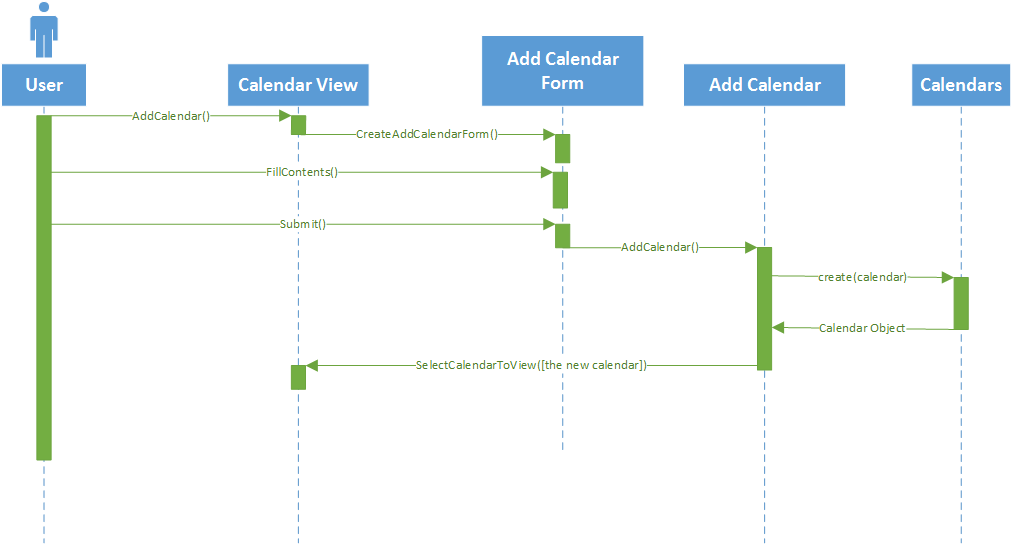
\includegraphics[scale=0.8]{figures/subscribe.png}
\end{figure}

\subsubsection{Add Event}
\begin{itemize}
\item \textbf{Entity}: User
\item \textbf{Boundary}: Calendars
\item \textbf{Control}: AddEvent
\end{itemize}

\clearpage
\begin{figure}[h]
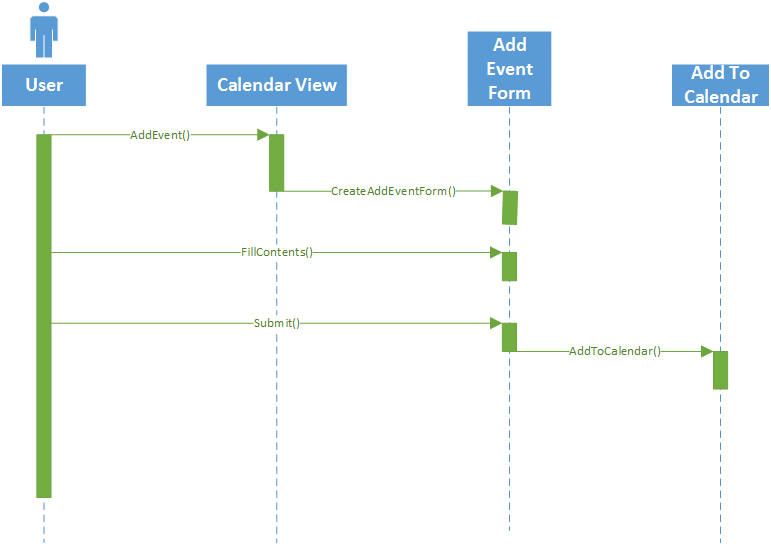
\includegraphics[scale=0.8]{figures/addevent.png}
\end{figure}

\subsubsection{Remove Event}
\begin{itemize}
\item \textbf{Entity}: User
\item \textbf{Boundary}: Calendars
\item \textbf{Control}: RemoveEvent
\end{itemize}

\begin{figure}[h]
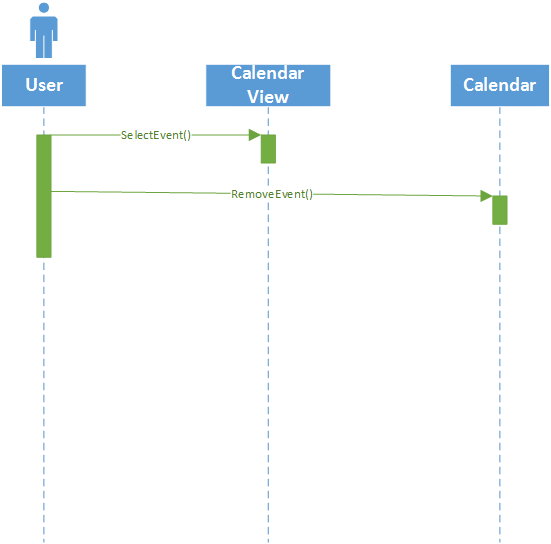
\includegraphics[scale=0.8]{figures/removeevent.png}
\end{figure}

\clearpage
\subsubsection{State machines}
\subsubsection{Subscribe calendar}
\begin{figure}[h]
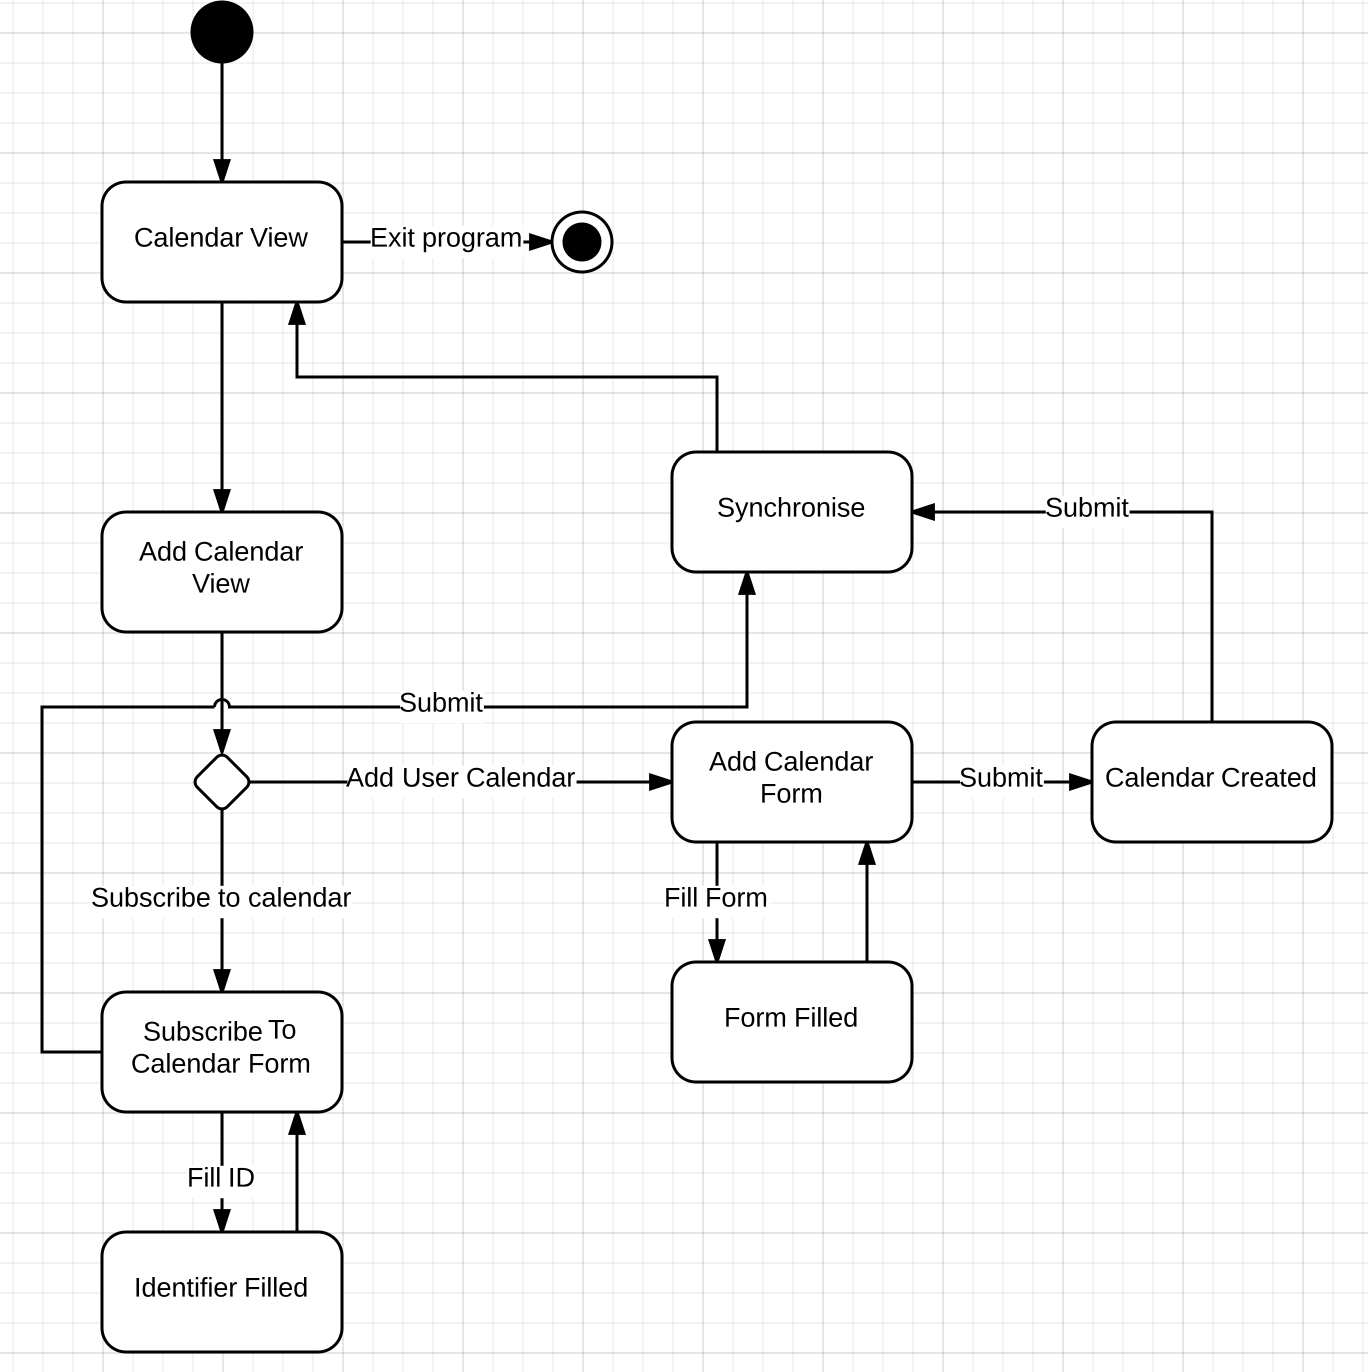
\includegraphics[scale=0.70]{figures/subcalendarstate.png}
\end{figure}

\clearpage
\subsubsection{Add event}
\begin{figure}[h]
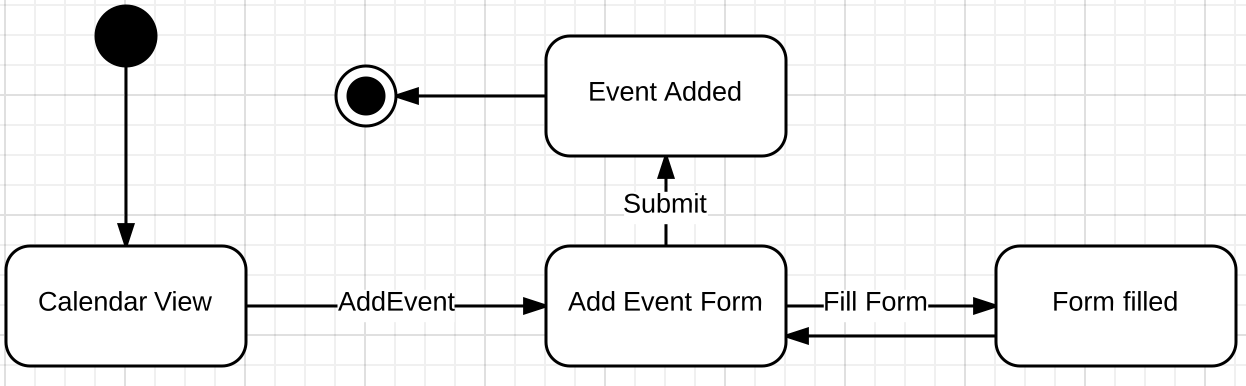
\includegraphics[scale=0.8]{figures/addeventstate.png}
\end{figure}

\clearpage
\subsubsection{Remove event}
\begin{figure}[h]
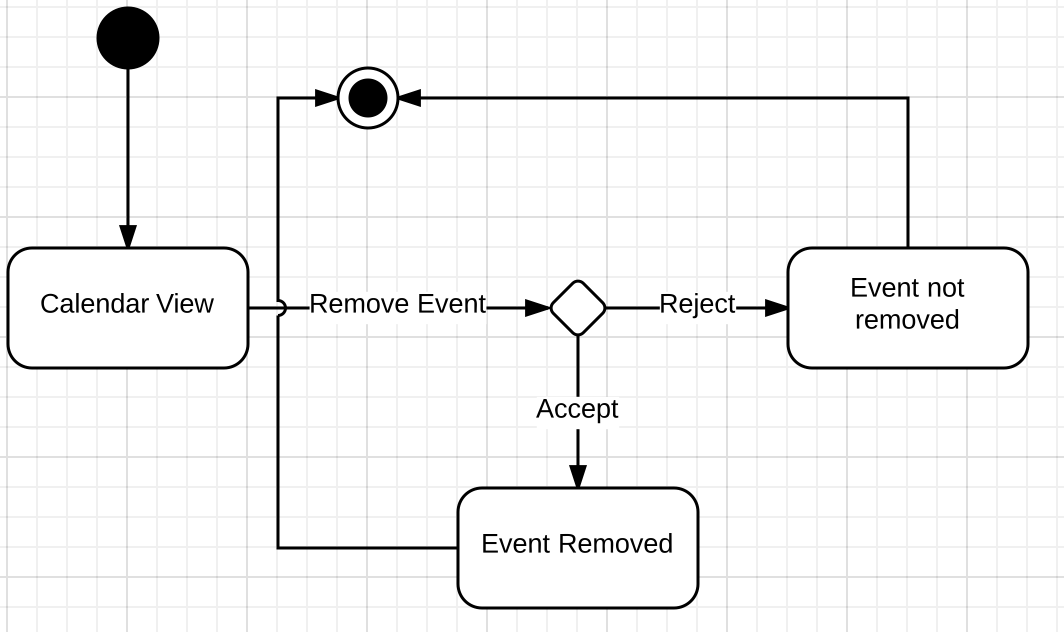
\includegraphics[scale=0.8]{figures/eventremovestate.png}
\end{figure}